% Options for packages loaded elsewhere
\PassOptionsToPackage{unicode}{hyperref}
\PassOptionsToPackage{hyphens}{url}
%
\documentclass[
]{article}
\usepackage{lmodern}
\usepackage{amssymb,amsmath}
\usepackage{ifxetex,ifluatex}
\ifnum 0\ifxetex 1\fi\ifluatex 1\fi=0 % if pdftex
  \usepackage[T1]{fontenc}
  \usepackage[utf8]{inputenc}
  \usepackage{textcomp} % provide euro and other symbols
\else % if luatex or xetex
  \usepackage{unicode-math}
  \defaultfontfeatures{Scale=MatchLowercase}
  \defaultfontfeatures[\rmfamily]{Ligatures=TeX,Scale=1}
  \ifxetex
    \usepackage{xeCJK}
    \setCJKmainfont[]{Microsoft YaHei}
  \fi
  \ifluatex
    \usepackage[]{luatexja-fontspec}
    \setmainjfont[]{Microsoft YaHei}
  \fi
\fi
% Use upquote if available, for straight quotes in verbatim environments
\IfFileExists{upquote.sty}{\usepackage{upquote}}{}
\IfFileExists{microtype.sty}{% use microtype if available
  \usepackage[]{microtype}
  \UseMicrotypeSet[protrusion]{basicmath} % disable protrusion for tt fonts
}{}
\makeatletter
\@ifundefined{KOMAClassName}{% if non-KOMA class
  \IfFileExists{parskip.sty}{%
    \usepackage{parskip}
  }{% else
    \setlength{\parindent}{0pt}
    \setlength{\parskip}{6pt plus 2pt minus 1pt}}
}{% if KOMA class
  \KOMAoptions{parskip=half}}
\makeatother
\usepackage{xcolor}
\IfFileExists{xurl.sty}{\usepackage{xurl}}{} % add URL line breaks if available
\IfFileExists{bookmark.sty}{\usepackage{bookmark}}{\usepackage{hyperref}}
\hypersetup{
  pdftitle={PhenoAsync},
  pdfauthor={Dongdong Kong},
  hidelinks,
  pdfcreator={LaTeX via pandoc}}
\urlstyle{same} % disable monospaced font for URLs
\usepackage[margin=1in]{geometry}
\usepackage{color}
\usepackage{fancyvrb}
\newcommand{\VerbBar}{|}
\newcommand{\VERB}{\Verb[commandchars=\\\{\}]}
\DefineVerbatimEnvironment{Highlighting}{Verbatim}{commandchars=\\\{\}}
% Add ',fontsize=\small' for more characters per line
\usepackage{framed}
\definecolor{shadecolor}{RGB}{248,248,248}
\newenvironment{Shaded}{\begin{snugshade}}{\end{snugshade}}
\newcommand{\AlertTok}[1]{\textcolor[rgb]{0.94,0.16,0.16}{#1}}
\newcommand{\AnnotationTok}[1]{\textcolor[rgb]{0.56,0.35,0.01}{\textbf{\textit{#1}}}}
\newcommand{\AttributeTok}[1]{\textcolor[rgb]{0.77,0.63,0.00}{#1}}
\newcommand{\BaseNTok}[1]{\textcolor[rgb]{0.00,0.00,0.81}{#1}}
\newcommand{\BuiltInTok}[1]{#1}
\newcommand{\CharTok}[1]{\textcolor[rgb]{0.31,0.60,0.02}{#1}}
\newcommand{\CommentTok}[1]{\textcolor[rgb]{0.56,0.35,0.01}{\textit{#1}}}
\newcommand{\CommentVarTok}[1]{\textcolor[rgb]{0.56,0.35,0.01}{\textbf{\textit{#1}}}}
\newcommand{\ConstantTok}[1]{\textcolor[rgb]{0.00,0.00,0.00}{#1}}
\newcommand{\ControlFlowTok}[1]{\textcolor[rgb]{0.13,0.29,0.53}{\textbf{#1}}}
\newcommand{\DataTypeTok}[1]{\textcolor[rgb]{0.13,0.29,0.53}{#1}}
\newcommand{\DecValTok}[1]{\textcolor[rgb]{0.00,0.00,0.81}{#1}}
\newcommand{\DocumentationTok}[1]{\textcolor[rgb]{0.56,0.35,0.01}{\textbf{\textit{#1}}}}
\newcommand{\ErrorTok}[1]{\textcolor[rgb]{0.64,0.00,0.00}{\textbf{#1}}}
\newcommand{\ExtensionTok}[1]{#1}
\newcommand{\FloatTok}[1]{\textcolor[rgb]{0.00,0.00,0.81}{#1}}
\newcommand{\FunctionTok}[1]{\textcolor[rgb]{0.00,0.00,0.00}{#1}}
\newcommand{\ImportTok}[1]{#1}
\newcommand{\InformationTok}[1]{\textcolor[rgb]{0.56,0.35,0.01}{\textbf{\textit{#1}}}}
\newcommand{\KeywordTok}[1]{\textcolor[rgb]{0.13,0.29,0.53}{\textbf{#1}}}
\newcommand{\NormalTok}[1]{#1}
\newcommand{\OperatorTok}[1]{\textcolor[rgb]{0.81,0.36,0.00}{\textbf{#1}}}
\newcommand{\OtherTok}[1]{\textcolor[rgb]{0.56,0.35,0.01}{#1}}
\newcommand{\PreprocessorTok}[1]{\textcolor[rgb]{0.56,0.35,0.01}{\textit{#1}}}
\newcommand{\RegionMarkerTok}[1]{#1}
\newcommand{\SpecialCharTok}[1]{\textcolor[rgb]{0.00,0.00,0.00}{#1}}
\newcommand{\SpecialStringTok}[1]{\textcolor[rgb]{0.31,0.60,0.02}{#1}}
\newcommand{\StringTok}[1]{\textcolor[rgb]{0.31,0.60,0.02}{#1}}
\newcommand{\VariableTok}[1]{\textcolor[rgb]{0.00,0.00,0.00}{#1}}
\newcommand{\VerbatimStringTok}[1]{\textcolor[rgb]{0.31,0.60,0.02}{#1}}
\newcommand{\WarningTok}[1]{\textcolor[rgb]{0.56,0.35,0.01}{\textbf{\textit{#1}}}}
\usepackage{graphicx,grffile}
\makeatletter
\def\maxwidth{\ifdim\Gin@nat@width>\linewidth\linewidth\else\Gin@nat@width\fi}
\def\maxheight{\ifdim\Gin@nat@height>\textheight\textheight\else\Gin@nat@height\fi}
\makeatother
% Scale images if necessary, so that they will not overflow the page
% margins by default, and it is still possible to overwrite the defaults
% using explicit options in \includegraphics[width, height, ...]{}
\setkeys{Gin}{width=\maxwidth,height=\maxheight,keepaspectratio}
% Set default figure placement to htbp
\makeatletter
\def\fps@figure{htbp}
\makeatother
\setlength{\emergencystretch}{3em} % prevent overfull lines
\providecommand{\tightlist}{%
  \setlength{\itemsep}{0pt}\setlength{\parskip}{0pt}}
\setcounter{secnumdepth}{5}
% https://github.com/rstudio/rmarkdown/issues/337
\let\rmarkdownfootnote\footnote%
\def\footnote{\protect\rmarkdownfootnote}

% https://github.com/rstudio/rmarkdown/pull/252
\usepackage{titling}
\setlength{\droptitle}{-2em}

\pretitle{\vspace{\droptitle}\centering\huge}
\posttitle{\par}

\preauthor{\centering\large\emph}
\postauthor{\par}

\predate{\centering\large\emph}
\postdate{\par}

\title{PhenoAsync}
\author{Dongdong Kong}
\date{2019/12/6}

\begin{document}
\maketitle

\hypertarget{r-markdown}{%
\subsection{R Markdown}\label{r-markdown}}

\begin{Shaded}
\begin{Highlighting}[]
\KeywordTok{load}\NormalTok{(}\StringTok{"INPUT/pheno_EVI_st95.rda"}\NormalTok{)}
\KeywordTok{load}\NormalTok{(}\StringTok{"INPUT/pheno_NDVI_st95.rda"}\NormalTok{)}
\KeywordTok{load}\NormalTok{(}\StringTok{"INPUT/pheno_LAI_st95.rda"}\NormalTok{)}
\KeywordTok{load}\NormalTok{(}\StringTok{"INPUT/pheno_gpp_st109.rda"}\NormalTok{)}

\NormalTok{sites =}\StringTok{ }\KeywordTok{names}\NormalTok{(lst_LAI)}

\NormalTok{melt_pheno <-}\StringTok{ }\ControlFlowTok{function}\NormalTok{(lst) \{}
\NormalTok{    res <-}\StringTok{ }\KeywordTok{foreach}\NormalTok{(}\DataTypeTok{l =}\NormalTok{ lst, }\DataTypeTok{i =} \KeywordTok{icount}\NormalTok{()) }\OperatorTok\StringTok{ }\NormalTok{\{}
        \CommentTok{# print(i)}
\NormalTok{        temp <-}\StringTok{ }\KeywordTok{map}\NormalTok{(l, }\StringTok{"pheno"}\NormalTok{) }\OperatorTok\StringTok{ }\KeywordTok{rm_empty}\NormalTok{()}
        \ControlFlowTok{if}\NormalTok{ (}\OperatorTok{!}\KeywordTok{is_empty}\NormalTok{(temp)) \{}
\NormalTok{            Ipaper}\OperatorTok{::}\KeywordTok{melt_list}\NormalTok{(temp, }\StringTok{"group"}\NormalTok{)}
\NormalTok{        \} }\ControlFlowTok{else} \OtherTok{NULL}
\NormalTok{    \} }\OperatorTok\StringTok{ }\KeywordTok{rm_empty}\NormalTok{()}
\NormalTok{    Ipaper}\OperatorTok{::}\KeywordTok{melt_list}\NormalTok{(res, }\StringTok{"site"}\NormalTok{)}
\NormalTok{\}}

\CommentTok{## MAIN SCRIPTS ----------------------------------------------------------------}
\NormalTok{sitename =}\StringTok{ }\NormalTok{sites[}\DecValTok{1}\NormalTok{]}
\NormalTok{df_gpp =}\StringTok{ }\KeywordTok{map}\NormalTok{(lst_pheno[sites], }\StringTok{"doy"}\NormalTok{) }\OperatorTok\StringTok{ }\KeywordTok{melt_tree}\NormalTok{(}\KeywordTok{c}\NormalTok{(}\StringTok{"site"}\NormalTok{, }\StringTok{"meth"}\NormalTok{))}

\NormalTok{lst_VI =}\StringTok{ }\KeywordTok{list}\NormalTok{(}\DataTypeTok{EVI =}\NormalTok{ lst_EVI, }\DataTypeTok{NDVI =}\NormalTok{ lst_NDVI, }\DataTypeTok{LAI =}\NormalTok{ lst_LAI)}
\NormalTok{df_VI =}\StringTok{ }\KeywordTok{map}\NormalTok{(lst_VI, melt_pheno) }\OperatorTok\StringTok{ }\NormalTok{Ipaper}\OperatorTok{::}\KeywordTok{melt_list}\NormalTok{(}\StringTok{"type_VI"}\NormalTok{)}

\CommentTok{# r <- lst_VI %>% map_depth(3, "pheno") %>% melt_tree(c("type_VI", "site", "group"))}
\CommentTok{# r <- lst_NDVI %>% map_depth(2, "pheno") %>% melt_tree(c("site", "group"))}
\CommentTok{# r <- lst_EVI %>% map_depth(2, "pheno") %>% melt_tree(c("site", "group"))}
\CommentTok{# r <- lst_LAI %>% map_depth(2, "pheno") %>% melt_tree(c("site", "group"))}
\CommentTok{# map(lst_VI, melt_pheno)}

\CommentTok{## 每年仅挑取最大GSL的season, GSL = TRS5.EOS - TRS5.SOS}
\NormalTok{filter_primary <-}\StringTok{ }\ControlFlowTok{function}\NormalTok{(df)\{}
\NormalTok{    df[, GSL }\OperatorTok{:}\ErrorTok{=}\StringTok{ }\NormalTok{TRS5.eos }\OperatorTok{-}\StringTok{ }\NormalTok{TRS5.sos]}
\NormalTok{    groups =}\StringTok{ }\NormalTok{.(type_VI, site, meth, group, origin) }\OperatorTok\StringTok{ }\KeywordTok{names}\NormalTok{() }\OperatorTok\StringTok{ }\KeywordTok{intersect}\NormalTok{(}\KeywordTok{names}\NormalTok{(df))}
\NormalTok{    I_sel <-}\StringTok{ }\NormalTok{df[, }\KeywordTok{order}\NormalTok{(}\OperatorTok{-}\NormalTok{GSL), groups]}\OperatorTok{$}\NormalTok{V1 }\OperatorTok{==}\StringTok{ }\DecValTok{1} \OperatorTok{&}\StringTok{ }\NormalTok{df}\OperatorTok{$}\NormalTok{GSL }\OperatorTok{>}\StringTok{ }\DecValTok{30}
\NormalTok{    df[I_sel, ]}
\NormalTok{\}}

\NormalTok{df_VI_prim  <-}\StringTok{ }\KeywordTok{filter_primary}\NormalTok{(df_VI)}
\NormalTok{df_gpp_prim <-}\StringTok{ }\KeywordTok{filter_primary}\NormalTok{(df_gpp)}
\end{Highlighting}
\end{Shaded}

\begin{Shaded}
\begin{Highlighting}[]
\NormalTok{df =}\StringTok{ }\KeywordTok{merge}\NormalTok{(}
    \KeywordTok{melt}\NormalTok{(df_VI_prim, }\KeywordTok{c}\NormalTok{(}\StringTok{"type_VI"}\NormalTok{, }\StringTok{"group"}\NormalTok{, }\StringTok{"site"}\NormalTok{, }\StringTok{"flag"}\NormalTok{, }\StringTok{"origin"}\NormalTok{, }\StringTok{"meth"}\NormalTok{), }\DataTypeTok{value.name =} \StringTok{"y_sim"}\NormalTok{),}
    \KeywordTok{melt}\NormalTok{(df_gpp_prim, }\KeywordTok{c}\NormalTok{(}\StringTok{"site"}\NormalTok{, }\StringTok{"flag"}\NormalTok{, }\StringTok{"origin"}\NormalTok{, }\StringTok{"meth"}\NormalTok{), }\DataTypeTok{value.name =} \StringTok{"y_obs"}\NormalTok{)}
    \CommentTok{# all.x = TRUE}
\NormalTok{)[, diff }\OperatorTok{:}\ErrorTok{=}\StringTok{ }\NormalTok{y_sim }\OperatorTok{-}\StringTok{ }\NormalTok{y_obs]}

\NormalTok{per_bad =}\StringTok{ }\KeywordTok{sum}\NormalTok{(}\KeywordTok{abs}\NormalTok{(df}\OperatorTok{$}\NormalTok{diff) }\OperatorTok{>=}\StringTok{ }\DecValTok{90}\NormalTok{, }\DataTypeTok{na.rm =} \OtherTok{TRUE}\NormalTok{)}\OperatorTok{/}\KeywordTok{nrow}\NormalTok{(df)}
\NormalTok{per_bad}
\end{Highlighting}
\end{Shaded}

\begin{verbatim}
## [1] 0.0557284
\end{verbatim}

Even trough we have dealed with growing season dividing very carefully,
there are still 5.5\% phenological metrics has a absolute error higher
than 90d. If absolute difference of \(y_{sim}\) and \(y_{obs}\) is high
that 90d (about 3 month), it might be introduced by the error of growing
season dividing. Hence, those phenological metrics are excluded when
calculating the goodness performance.

\hypertarget{including-plots}{%
\subsection{Including Plots}\label{including-plots}}

You can also embed plots, for example:

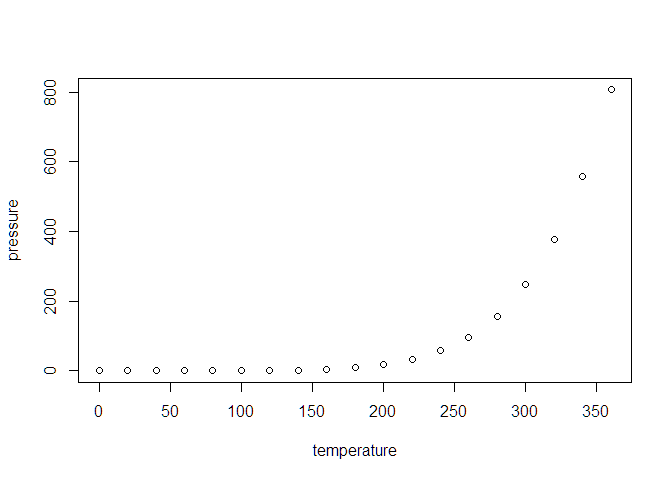
\includegraphics{PhenoAsync_result_files/figure-latex/pressure-1.pdf}

Note that the \texttt{echo\ =\ FALSE} parameter was added to the code
chunk to prevent printing of the R code that generated the plot.

\end{document}
